\documentclass{article}

\usepackage{amsthm}
\usepackage{amsmath}
\usepackage{amssymb}
\usepackage{enumitem}
\usepackage{todonotes}
\usepackage{setspace}
\usepackage{hyperref}
\usepackage[spanish]{cleveref}

\usepackage{tikz}
\usetikzlibrary{shapes.geometric, arrows}
\tikzstyle{caja} = [rectangle, rounded corners, minimum width=2cm, minimum height=1cm,align=center, draw=black, fill=black!10]
\tikzstyle{solotexto} = [align=center]
\tikzstyle{arrow} = [thick,->,>=stealth]

\theoremstyle{definition}
\newtheorem{definition}{Definici\'on}%[section]
\newtheorem{example}{Ejemplo}%[section]

\title{El modelo de aprendizaje PAC}
\date{Enero 2022.}
\author{Agust\'in E. Martinez Su\~n\'e}

\begin{document}

\maketitle

Trabajo final para la materia \emph{M\'etodos probabil\'isticos avanzados y Machine Learning} a cargo del Prof. Pablo Groisman.
\section{Introducci\'on}

Machine learning es un \'area extremadamente diversa y compleja. M\'etodos estad\'isticos de regresi\'on, algoritmos que utilizan redes neuronales, paseos al azar en grafos, problemas de optimizaci\'on, y muchos otros problemas y m\'etodos pueden enmarcarse en el \'area de aprendizaje autom\'atico. Ser\'ia interesante contar con una misma teor\'ia o marco conceptual para comparar y analizar esta diversidad de herramientas. El \emph{modelo de aprendizaje PAC}, propuesto originalmente por Leslie Valiant en 1984\cite{valiant:ca84}, es un aporte en esta direcci\'on y sienta las bases de lo que hoy se conoce como \emph{Computational Learning Theory}. Para darse una idea del impacto de esta propuesta, al menos en la comunidad de Ciencias de la Computaci\'on, puede verse el texto que acompa\~na la entrega del \emph{Premio Turing} a Valiant en el a\~no 2010:
\begin{quote}
    For transformative contributions to the theory of computation, including the theory of probably approximately correct (PAC) learning, (\dots)
\end{quote}

Este texto nos da una pista sobre la perspectiva particular desde la que Valiant encara el problema: la \emph{teor\'ia de la computaci\'on}, y en particular, la \emph{teor\'ia de la complejidad computacional}. El objetivo de este trabajo es dar una introducci\'on a la teor\'ia iniciada por Valiant, enfatizando esta perspectiva computacional.

En la secci\'on \ref{sec:computation} introducimos de manera informal conceptos b\'asicos de complejidad computacional, en la secci\'on \ref{sec:pac} definimos formalmente las principales nociones del modelo de aprendizaje PAC, en la secci\'on \ref{sec:var} exploramos algunas variantes de la definici\'on original y en la secci\'on \ref{sec:conclusiones} damos unas breves conclusiones.
Adem\'as del art\'iculo original de Valiant, las principales fuentes consultadas para las definiciones principales fueron los libros \emph{Foundations of Machine Learning}\cite{mohri18} y \emph{An Introduction to Computational Learning Theory}\cite{kearns94}.

\section{Teor\'ia de la complejidad computacional}
\label{sec:computation}

En esencia, la teor\'ia de complejidad computacional estudia el v\'inculo entre problemas computacionales y los algoritmos que los resuelven y brinda herramientas para analizar y categorizar dichos problemas y algoritmos. Comenzamos definiendo uno de los tipos de problemas computacionales m\'as b\'asicos.

\begin{definition}[Problema de decisi\'on]
\label{def:decision}
Dado un conjunto de \emph{inputs} $X$, un problema de decisi\'on se puede describir como una funci\'on total $f : X \to \{0, 1\}$. En otras palabras, un problema de decisi\'on requiere que, para cada input, se de una respuesta por s\'i o por no.

En ese contexto, vamos a decir que un \emph{algoritmo} $A$ resuelve el problema si y s\'olo si para cada $x \in X$, el algoritmo $A$ con entrada $x$ termina en una cantidad finita de pasos con una salida $y$ tal que $f(x) = y$.
\end{definition}

\begin{example}
    Un cl\'asico ejemplo de problema de decisi\'on es el \emph{test de primalidad} en el que dado un natural $n$ se debe responder si $n$ es primo o no.
\end{example}

Para un mismo problema de decisi\'on pueden existir distintos algoritmos que lo resuelvan satisfactoriamente, y es de inter\'es tener alguna herramienta para compararlos. La herramienta can\'onica para hacerlo es el llamado \emph{costo computacional} o \emph{complejidad temporal}, que agrupa los algoritmos en grandes clases seg\'un la cantidad de operaciones b\'asicas que requiere una ejecuci\'on del mismo.

\begin{definition}[Algoritmo polinomial]
    \label{def:algopoly}
    Sea $A$ un algoritmo que toma valores de entrada $x \in X$, decimos que $A$ es un algoritmo polinomial si el costo computacional asociado a $A$ crece polinomialmente con $x$. Es decir, si dado $x$ de tama\~no $n$, la cantidad de pasos de ejecuci\'on de $A$ con entrada $x$ es $\mathit{poly}(x)$, donde $\mathit{poly} : \mathbb{N} \to \mathbb{N}$ es un polinomio.
\end{definition}

Hay ciertos detalles formales que no estamos explicitando en estas definiciones ya que no es el objetivo de este trabajo. Por ejemplo, se deber\'ia definir formalmente la noci\'on de algoritmo, de costo computacional, y se deber\'ia indicar formalmente que cada elemento del conjunto de inputs $X$ es representable de manera finita. Esto suele definirse apelando a la \emph{teor\'ia de lenguajes formales} y a alg\'un modelo de computo espec\'ifico como la \emph{m\'aquina de turing}. El lector interesado puede encontrar estas definiciones en la bibliograf\'ia cl\'asica del \'area \cite{cormen01,hopcroft79}. 
Ahora estamos en condiciones de definir clases de complejidad de problemas.

\begin{definition}[Clase de complejidad P]
    \label{def:classp}
    Un problema de decisi\'on $D$ est\'a en la clase de complejidad $\mathbf{P}$ (tambi\'en llamada $\mathbf{PTIME}$) si y s\'olo si existe un algoritmo polinomial que resuelve $D$.
\end{definition}

El concepto de algoritmo polinomial intenta capturar desde la teor\'ia el fen\'omeno esencialmente pr\'actico de que hay ciertos algoritmos que podemos ejecutar en una computadora de manera \emph{eficiente} en un tiempo razonable y hay otros que no. Por extensi\'on, se dice que un problema es \emph{tratable} si est\'a en $\mathbf{P}$ y es \emph{intratable} si no.\footnote{Esta interpretaci\'on de las clases de complejidad no est\'a excenta de pol\'emica. Existen problemas que est\'an en $\mathbf{P}$ para los cuales no tenemos implementaciones pr\'acticas eficientes y existen problemas que no parecen estar en $\mathbf{P}$ para los cu\'ales s\'i las tenemos. Se puede encontrar una discusi\'on del tema en \cite{vardi:ca10}.}

Como adelantamos previamente, el objetivo de esta visita r\'apida a la teor\'ia de complejidad computacional es facilitar la introducci\'on de los conceptos del modelo PAC desde una perspectiva computacional. Para eso, debemos observar que las preguntas esenciales detr\'as de las definiciones presentadas son:
\begin{itemize}
    % \item \emph{?`Cu\'al es el problema computacional que se quiere resolver?}
    \item \emph{?`C\'omo var\'ia la cantidad de pasos de ejecuci\'on de un algoritmo a medida que aumenta el tama\~no de los datos de entrada?}
    \item \emph{?`C\'omo distinguimos aquellos problemas que se pueden resolver de manera "razonable" por una computadora de aquellos que no?}
\end{itemize}

\section{Bases del aprendizaje PAC}
\label{sec:pac}

En este contexto, el problema computacional de inter\'es es el problema de aprendizaje, entendido como el problema de construir una \emph{hip\'otesis} o \emph{clasificador} que generalice las \emph{etiquetas} de una \emph{muestra} tomada de una distribuci\'on de probabilidad. En este escenario, el algoritmo que nos interesa estudiar es aquel que toma como entrada un conjunto de datos etiquetados y da como salida una \emph{hip\'otesis}.

\begin{center}
    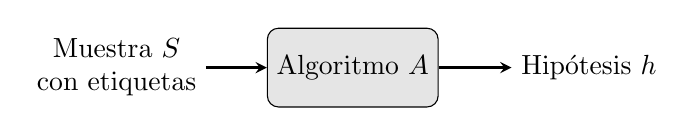
\begin{tikzpicture}[node distance=3cm]
        \node (data) [solotexto] {Muestra $S$ \\ con etiquetas};
        \node (alg) [caja, right of=data] {Algoritmo $A$};
        \node (hip) [solotexto, right of = alg] {Hip\'otesis $h$};
        
        \draw [arrow] (data) -- (alg);
        \draw [arrow] (alg) -- (hip);
    \end{tikzpicture}
\end{center}

Continuando con la analog\'ia con la secci\'on anterior, la pregunta central que el modelo de aprendizaje PAC intenta responder es:

\begin{center}
    \emph{?`C\'omo var\'ia el tama\~no de la muestra necesaria para el aprendizaje a medida que exijo mayor precisi\'on en las predicciones de la hip\'otesis?}    
\end{center}

A continuaci\'on vamos dar la definici\'on principal del modelo PAC de manera informal y luego iremos construyendo de manera rigurosa las herramientas necesarias para formalizarla.

\begin{definition}[Noci\'on informal de algoritmo PAC]
    Dado $A$ un algoritmo de aprendizaje que toma una muestra $S$ de tama\~no $m$ y devuelve una hip\'otesis $h$, se puede medir la \emph{confianza} y la \emph{precisi\'on} de $h$. Decimos que $A$ es un algoritmo PAC si y s\'olo si, al hacer crecer la \emph{precision} y la \emph{confianza} requeridas, el tama\~no $m$ que se necesita crece a lo sumo polinomialmente.
\end{definition}

Para avanzar en definir formalmente un problema de aprendizaje necesitamos introducir la noci\'on de clase de conceptos.

\begin{definition}[Concepto y clase de conceptos]
    Sea $\mathcal{X}$ el \emph{input space} y $\mathcal{Y}$ el conjunto de \emph{etiquetas} o \emph{target values} decimos que un \emph{concepto} $c$ es un mapeo de $\mathcal{X}$ a $\mathcal{Y}$ (lo notamos $c : \mathcal{X} \to \mathcal{Y}$). Una \emph{clase de conceptos} $\mathcal{C}$ es un conjunto de conceptos que nos interesa aprender.
\end{definition}

\begin{example}
    
    Imaginemos que nuestras instancias de entrada son puntos en el plano y que la tarea es aprender el conjunto de puntos interiores de un tri\'angulo que desconocemos. En ese caso:
    \begin{itemize}
        \item $\mathcal{X} = \mathbb{R}^2$, el input space es todo el plano real,
        \item $\mathcal{Y} = \{0, 1\}$, cada etiqueta indica si el punto se encuentra dentro del tri\'angulo o no,
        \item Cualquier tri\'angulo del plano se puede caracterizar como un concepto $c : \mathcal{X} \to \mathcal{Y}$,
        \item la clase de conceptos $\mathcal{C}$ adecuada, es el conjunto de todos los $c : \mathcal{X} \to \mathcal{Y}$ que caracterizan triangulos del plano.
    \end{itemize}
    En este ejemplo estamos frente a un problema de \emph{clasificaci\'on binaria} ya que $\mathcal{Y}$ contiene s\'olo dos etiquetas.

\end{example}

A continuaci\'on definimos formalmente el problema de aprendizaje.

\begin{definition}[Problema de aprendizaje]
    Sean un input space $\mathcal{X}$, un conjunto de etiquetas $\mathcal{Y}$, una clase de conceptos $C$ (de la forma $c : \mathcal{X} \to \mathcal{Y}$) y una distribuci\'on de probabilidad $\mathcal{D}$ sobre $\mathcal{X}$. El problema de aprendizaje es, dados una muestra $S = \{x_1, \dots, x_m\} \sim \mathcal{D}^m$ y las correspondientes etiquetas $\{c(x_1), \dots, c(x_m)\}$ asociadas, seg\'un un concepto $c \in \mathcal{C}$, construir una hip\'otesis $h_{S} : \mathcal{X} \to \mathcal{Y}$ que aproxime $c$ en futuros inputs tomados de $\mathcal{D}$.
    
    Un algoritmo de aprendizaje $A$ considera un conjunto fijo $\mathcal{H}$ de posibles conceptos, llamado \emph{conjunto de hip\'otesis}. La distribuci\'on $\mathcal{D}$, si bien es fija, es desconocida para el algoritmo de aprendizaje.
    %$\mathcal{H}$ no necesariamente coincide con $\mathcal{C}$.
\end{definition}

\begin{center}
    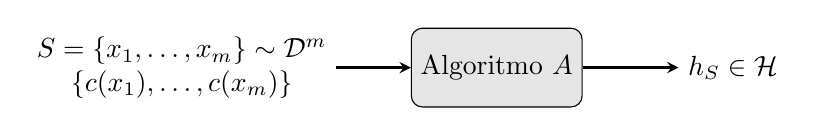
\begin{tikzpicture}[node distance=3cm]
        \node (data) [solotexto] {$S = \{x_1, \dots, x_m\} \sim \mathcal{D}^m$ \\ $\{c(x_1), \dots, c(x_m)\}$};
        \node (alg) [caja, right of=data, xshift=1cm] {Algoritmo $A$};
        \node (hip) [solotexto, right of = alg] {$h_S \in \mathcal{H}$};
        
        \draw [arrow] (data) -- (alg);
        \draw [arrow] (alg) -- (hip);
    \end{tikzpicture}
\end{center}

Dado un problema de aprendizaje y un algoritmo espec\'ifico que lo resuelve, la calidad la hip\'otesis que devuelve depende del error de generalizaci\'on.

\begin{definition}[Error de generalizaci\'on]
    Dada una hip\'otesis $h \in \mathcal{H}$, un concepto $c \in \mathcal{C}$ y una distribuci\'on subyacente $\mathcal{D}$, el \emph{error de generalizaci\'on} se define como: 
    $$
    R(h) = \mathbb{P}_{x \sim \mathcal{D}}[h(x) \neq c(x)]
    $$
\end{definition}

Ahora s\'i est\'an todos los ingredientes para la definici\'on central de la teor\'ia: Algoritmo \emph{Probably Approximately Correct}.

\begin{definition}[Algoritmo PAC]
    \label{def:pac}
    Dado un algoritmo de aprendizaje $A$ que intenta aprender una clase de conceptos $\mathcal{C}$, decimos que es un \emph{algoritmo PAC} si y s\'olo si existe un polinomio $p(\cdot, \cdot)$ tal que para todo $0 < \epsilon < \frac{1}{2}$, $0 < \delta < 1$, concepto $c \in \mathcal{C}$, y distribuci\'on de probabilidad $\mathcal{D}$ sobre $\mathcal{X}$, si se toma una muestra de tama\~no $m \geq p(\epsilon^{-1}, \delta^{-1})$, entonces
    $$
    \mathbb{P}_{S\sim\mathcal{D}^m}[R(h_S) \leq \epsilon] \geq 1 - \delta
    $$
\end{definition}

Valores chicos de $\epsilon$ denotan altos niveles de precisi\'on de la hip\'otesis $h_S$, valores chicos de $\delta$ denotan altos niveles de confianza en dicha precisi\'on. Esto explica por qu\'e el polinomio $p$ se aplica sobre $\epsilon^{-1}$ y $\delta^{-1}$. La terminolog\'ia \emph{Probably Approximately Correct (PAC)} refiere a estos conceptos: ``probably'' por la confianza y ``approximately correct'' por la precisi\'on.
Por simplicidad, en la definici\'on anterior se omitieron dos factores que tambi\'en intervienen en el crecimiento del polinomio $p$: el costo de representaci\'on de un elemento $x \in \mathcal{X}$ y el costo de representaci\'on de un concepto $c \in \mathcal{C}$.

Bajo la luz de esta definici\'on, podemos comparar distintos algorimtos PAC seg\'un el tama\~no de la muestra que necesitan para aprender un concepto de manera exitosa.

\begin{definition}[Sample complexity]
    Dado un algoritmo $A$ de aprendizaje PAC, llamaremos \emph{complejidad de muestra} de $A$ al polinomio $p$ m\'as chico asociado a $A$ seg\'un la definici\'on \ref{def:pac}.
\end{definition}

Finalmente, estamos en condiciones de definir cu\'ales son aquellos problemas de aprendizaje que se pueden resolver de manera ``razonable'' seg\'un el modelo PAC. Retomando la comparaci\'on con las ideas b\'asicas de complejidad computacional introducidas en la secci\'on anterior, proponemos pensar esta definici\'on en analog\'ia con la de clase de complejidad $\mathbf{P}$.

\begin{definition}[PAC learnable]
    Dada una clase de conceptos $\mathcal{C}$, diremos que $\mathcal{C}$ es \emph{PAC learnable} si y s\'olo si existe un algoritmo de aprendizaje PAC para $\mathcal{C}$.
\end{definition}

A continuaci\'on veremos en detalle un ejemplo de un problema que se puede demostrar PAC learnable. 

\begin{example}[Los intervalos son PAC learnable] 

    La tarea es aprender un intervalo de la recta real a partir de una muestra de puntos. En este caso tenemos:
    \begin{itemize}
        \item $\mathcal{X} = \mathbb{R}$, el input space son los puntos de la recta real,
        \item $\mathcal{Y} = \{0, 1\}$, cada etiqueta indica si el punto se encuentra dentro del intervalo o no,
        \item La clase de conceptos $\mathcal{C}$ son todas las $c : \mathcal{X} \to \mathcal{Y}$ que son funciones caracter\'isticas de un intervalo.
    \end{itemize}

    Dada una muestra de puntos $S = \{x_1, \dots, x_m\}$ con etiquetas $\{c(x_1), \dots, c(x_m)\}$, proponemos el siguiente algoritmo: 
    \begin{enumerate}
        \item tomar $a_1 = \min \{x \mid x \in S, c(x) = 1\}$, el valor m\'as chico de la muestra que est\'a dentro del intervalo,
        \item tomar $b_1 = \max \{x \mid x \in S, c(x) = 1\}$, el valor m\'as grande de la muestra que est\'a dentro del intervalo,
        \item devolver como hip\'otesis $h_S$ la funci\'on caracter\'istica del intervalo $[a_1, b_1]$.
    \end{enumerate}

    Para probar que es un algoritmo PAC tomamos cualquier $\epsilon, \delta$ y distribuci\'on $\mathcal{D}$ sobre $\mathcal{X}$, y debemos deducir el tama\~no de muestra $m$ que satisface la condici\'on $\mathbb{P}_{S\sim\mathcal{D}^m}[R(h_S) \leq \epsilon] \geq 1 - \delta$, o lo que es equivalente $\mathbb{P}_{S\sim\mathcal{D}^m}[R(h_S) \geq \epsilon] \leq \delta$

    Si el intervalo correcto que se debe aprender es $I = [a_0, b_0]$, el error de generalizaci\'on $R(h_S)$ en este caso es $\mathbb{P}_{x \sim \mathcal{D}}[x \in I \setminus h_S]$ ya que el \'unico caso en que la hip\'otesis falla es cuando un punto de $I$ se clasifica como negativo. 
    Sabemos que $h_S \subseteq I$, ya que los extremos $a_1$ y $b_1$ de $h_S$ con certeza est\'an dentro del intervalo. 
    Es decir, sabemos que $a_0 < a_1 < b_1 < b_0$, por lo tanto, podemos reescribir el error de generalizaci\'on como 
    $$\mathbb{P}_{x \sim \mathcal{D}}(a_0 < x < a_1) + \mathbb{P}_{x \sim \mathcal{D}}(b_1 < x < b_0)$$
    Queremos acotar esta suma por $\epsilon$, para eso vamos a acotar cada t\'ermino por $\epsilon/2$,
    $$\mathbb{P}_{x \sim \mathcal{D}}(a_0 < x < a_1) \geq \epsilon/2$$
    Esta probabilidad va a depender del valor $a_1$ que haya seleccionado nuestro algoritmo. Tomemos $a^\prime$ tal que 
    $$\mathbb{P}_{x \sim \mathcal{D}}(a_0 < x < a^\prime) = \epsilon/2$$
    La desigualdad $\mathbb{P}_{x \sim \mathcal{D}}(a_0 < x < a_1) \geq \epsilon/2$ se cumple si y s\'olo si $a_1 \geq a^\prime$ y, por la forma en que funciona el algoritmo, esto sucede si ning\'un punto $y$ de la muestra $S$ cumple $a_0 < y < a^\prime$. La probabilidad de que un \'unico punto no este dentro del intervalo es $(1 - \epsilon/2)$, por la forma en que elegimos $a^\prime$. La probabilidad para $m$ puntos es $(1 - \epsilon/2)^m$. El razonamiento para el otro t\'ermino es an\'alogo, $\mathbb{P}_{x \sim \mathcal{D}}(b_1 < x < b_0) \geq \epsilon/2$ se cumple con probabilidad $(1 - \epsilon/2)^m$. 
    
    Repasando el razonamiento:
    \begin{align*}
        & \mathbb{P}_{S\sim\mathcal{D}^m}(R(h_S) \geq \epsilon) = \mathbb{P}_{S\sim\mathcal{D}^m}( \mathbb{P}_{x \sim \mathcal{D}}(a_0 < x < a_1) + \mathbb{P}_{x \sim \mathcal{D}}(b_1 < x < b_0) \geq \epsilon) \\
        & \quad \text{Por definici\'on de } R(h_S) \\
        \leq\ & \mathbb{P}_{S\sim\mathcal{D}^m}\big(\mathbb{P}_{x \sim \mathcal{D}}(a_0 < x < a_1) \geq \epsilon/2 \ \bigcup \ \mathbb{P}_{x \sim \mathcal{D}}(b_1 < x < b_0) \geq \epsilon/2\big) \\
        & \quad \text{Por inclusi\'on de eventos. Si la suma es mayor a $\epsilon$, entonces} \\
        & \quad \text{con certeza alguno de los dos sumandos es mayor a $\epsilon/2$.} \\
        \leq\ & \mathbb{P}_{S\sim\mathcal{D}^m}\big(\mathbb{P}_{x \sim \mathcal{D}}(a_0 < x < a_1) \geq \epsilon/2 \big) + \mathbb{P}_{S\sim\mathcal{D}^m}\big(\mathbb{P}_{x \sim \mathcal{D}}(b_1 < x < b_0) \geq \epsilon/2\big) \\
        & \quad \text{Por cota superior de la probabilidad de la union.} \\
        \leq\ & (1-\epsilon/2)^m + (1-\epsilon/2)^m \\
        & \quad \text{Por el razonamiento que hicimos en el parrafo anterior.} \\
    \end{align*}

Lo que resta ahora es acotar esta \'ultima expresi\'on por $\delta$ y resolver para $m$:
$$
2 (1-\epsilon/2)^m \leq \delta
$$

Usando el hecho de que $(1-x) \leq e^{-x}$ podemos acotar $(1-\epsilon/2)$, y resolver, en cambio, la siguiente desigualdad:
$$
2 e^{-m\epsilon/2} \leq \delta
$$

Basta tomar $m \geq (2/\epsilon \log(2/\delta))$. Si bien $(2/\epsilon \log(2/\delta))$ no es estrictamente un polinomio por el factor logar\'itmico, puede acotarse superiormente por un polinomio y este cumple el rol de la cota deseada.

\end{example}


\section{Variantes del aprendizaje PAC}

En esta secci\'on veremos dos variantes de la definici\'on de aprendizaje PAC que consideramos relevantes. No pretende ser una muestra extensiva o representativa de las distintas extensiones que se han propuesto para la definici\'on pero s\'i sirven de introducci\'on a la forma en que se puede pensar modificaciones que sean de utilidad para distintos escenarios.

\label{sec:var}

\subsection{PAC learning agn\'ostico}
La definici\'on presentada hasta el momento asume que, dado un input $x$, la etiqueta $y$ asociada es determin\'istica. Pero en muchos problemas de aprendizaje no supervisado esto no es cierto, sino que la distribuci\'on $\mathcal{D}$ se define sobre los pares $\mathcal{X} \times \mathcal{Y}$. 

\begin{example} Supongamos el problema de intentar predecir el nombre de pila de una persona a partir del g\'enero y del a\~no y ciudad de nacimiento. En este caso la etiqueta no es una funci\'on determin\'istica, para una misma combinaci\'on de g\'enero y a\~no y ciudad de nacimiento puede haber distintos datos de personas con nombres distintos. Sin embargo s\'i podemos estudiar la distribuci\'on de probabilidad que siguen estas etiquetas.
    
\end{example}

En estos escenarios la muestra de entrenamiento es de la forma
$$
S = \{(x_1, y_1), \dots, (x_m, y_m)\} \sim \mathcal{D}^m
$$

y debemos redefinir el error de generalizaci\'on de la siguiente manera.

\begin{definition}[Error de generalizaci\'on]
    Dada una hip\'otesis $h \in \mathcal{H}$, y una distribuci\'on $\mathcal{D}$, el \emph{error de generalizaci\'on} se define como: 
    $$
    R(h) = \mathbb{P}_{(x,y) \sim \mathcal{D}}[h(x) \neq y]
    $$
\end{definition}

En este contexto, la extensi\'on del framework se conoce como PAC learning \emph{agn\'ostico}.

\begin{definition}[PAC learning agn\'ostico]
    \label{def:pac-agnostico}
    Sea $\mathcal{H}$ el conjunto de hip\'otesis. Decimos que $A$ es un algoritmo de aprendizaje PAC agn\'ostico si y s\'olo si existe un polinomio $p(\cdot, \cdot)$ tal que para todo $0 < \epsilon < \frac{1}{2}$, $0 < \delta < 1$, y distribuci\'on de probabilidad $\mathcal{D}$ sobre $\mathcal{X} \times \mathcal{Y}$, si se toma una muestra de tama\~no $m \geq p(\epsilon^{-1}, \delta^{-1})$, entonces
    $$
    \mathbb{P}_{S\sim\mathcal{D}^m}[R(h_S) - \min_{h \in \mathcal{H}} R(h) \leq \epsilon] \geq 1 - \delta
    $$
\end{definition}

Mientras en la definici\'on original se ped\'ia que el error de $h_S$ sea menor o igual a $\epsilon$, en este caso lo que se pide acotar es la diferencia entre el error de $h_S$ y el error de la hip\'otesis \'optima. Esto se debe a que la hip\'otesis perfecta podr\'ia no existir porque la etiqueta de un punto en el \emph{input} no necesariamente es determin\'istica. En caso de que s\'i sea una funci\'on determin\'istica estamos en el caso de la definici\'on original y el error de la hip\'otesis \'optima es cero.

\subsection{PAC learning d\'ebil}

% En la definici\'on \cref{def:pac} introdujimos el polinomio $p$ que toma la precisi\'on $\epsilon^{-1}$ y la confianza $\delta^{-1}$. Dijimos que estabamos omitiendo dos factores, que ahora debemos explicitar: 
% \begin{itemize}
%     \item $O(n)$ el costo de representaci\'on de un elemento $x \in \mathcal{X}$ y
%     \item $\mathit{size}(c)$ el costo de representaci\'on de un concepto $c \in \mathcal{C}$.
% \end{itemize}

% Esto hace que la cota para el tama\~no de las muestra sea 
% $$
% m \geq p(\epsilon^{-1}, \delta^{-1}, n, \mathit{size}(c))
% $$

Observando nuevamente la definici\'on original \ref{def:pac}, la cota que venimos utilizando para el tama\~no de la muestra es $m \geq p(\epsilon^{-1}, \delta^{-1})$. Como ya mencionamos, la principal consecuencia de esta cota es que s\'olo permite que $m$ crezca polinomialmente a medida que crece la precisi\'on $\epsilon^{-1}$ y la confianza $\delta^{-1}$. 
Podemos definir un modelo m\'as d\'ebil que no requiera al algoritmo aprender una hip\'otesis con precisi\'on arbitrariamente grande, sino que requiera que la precisi\'on sea al menos mejor que adivinar al azar.

\begin{definition}[Algoritmo PAC d\'ebil]
    \label{def:pac-debil}
    Dado un algoritmo de aprendizaje $A$ que intenta aprender una clase de conceptos $\mathcal{C}$, decimos que es un algoritmo PAC \emph{d\'ebil} si y s\'olo si existe un polinomio $p(\cdot)$ tal que para todo $0 < \delta < 1$, concepto $c \in \mathcal{C}$, y distribuci\'on de probabilidad $\mathcal{D}$ sobre $\mathcal{X}$, si se toma una muestra de tama\~no $m \geq p(\delta^{-1})$, entonces
    $$
    \mathbb{P}_{S\sim\mathcal{D}^m}\big(R(h_S) < \frac{1}{2}\big) \geq 1 - \delta
    $$
\end{definition}

Est\'a definici\'on se vincula con el problema de \emph{boosting}: ¿c\'omo construir un algoritmo de aprendizaje de alta precisi\'on utilizando algoritmos de precisi\'on baja?. En t\'erminos te\'oricos la pregunta pertinente es: dado un problema de aprendizaje para el que se cuenta con un algoritmo PAC d\'ebil $A$, ¿se puede construir un algoritmo PAC \emph{fuerte} $A'$ (en el sentido de la definici\'on original) para el mismo problema? La respuesta es positiva y fue dada por Schapire en 1990 \cite{schapire:ml-5_2}. Esto abri\'o una rama de investigaci\'on que estudia distintos algoritmos de boosting para mejorar la performance combinando el output de distintos \emph{weak learners}.

\section{Conclusiones}
\label{sec:conclusiones}

En este trabajo dimos una introducci\'on al \'area de \emph{computational learning theory}. Vimos que este \'area toma la perspectiva de la teor\'ia de complejidad computacional para razonar sobre algoritmos de aprendizaje. La pregunta b\'asica que ordena estos an\'alisis es c\'omo var\'ia el tama\~no de la muestra necesaria para el aprendizaje a medida que se le requiere mayor precisi\'on al modelo aprendido.

A trav\'es de un ejemplo de algoritmo PAC vimos la forma en que las definiciones te\'oricas pueden ser puestas en pr\'actica. Finalmente, introdujimos algunas variantes de la definci\'on original que permiten extenderla para distintos escenarios y que fueron abriendo nuevas preguntas de investigaci\'on en el \'area.

\bibliographystyle{abbrv}
\bibliography{zoterolib}

\end{document}
